\section{Conception de la solution}

\subsection{Architecture de la solution}

    \subsubsection{Web Service}

    \subsubsection{Application Android}
Le développement du client mobile a suivi le schéma classique de conception d’une application Android. Pour rappel les objectifs initiaux majeurs de ce client étaient de pouvoir récupérer des données sur un web service, les exploiter, les afficher à l’utilisateur et enfin retourner des données au service en question. De façon général la solution Android s’organise en deux projets directeurs : les tests et l’implémentation de l’application. 

Il n’a pas choisi ici de faire du développement dirigé par les tests car la technologie Android était dans le cadre de ce projet une découverte et il aurait était hasardeux de définir des tests Java sur les concepts Android. Les tests ont donc ici vocation à valider les mécaniques métiers a posteriori ainsi que le bon fonctionnement et l’intégrité de l’application au fur et à mesure de l’ajout de fonctionnalités. La partie relative aux tests se subdivise en deux autres : les tests unitaires et les tests instrumentés. Les premiers sont plutôt classiques et permettent de tester les mécaniques métiers et de vérifier tout ce qui est mockable, autrement dit simulable. Toutefois, il y a certains aspects dans un programme Android qu’il n’est pas possible de mocker sans enlever l’intérêt du test. Nous parlons ici de fonctionnalités s’appuyant intrinsèquement sur le système Android comme les appels réseaux, le GPS, l’écran, etc. Il est nécessaire dès lors que l’on veut simuler une fonctionnalité Android même basique, de simuler tout un système Android. D’où l’intérêt de la deuxième catégorie de tests : les tests instrumentés. Ceux-ci vont être exécutés sur un émulateur Android directement afin de pouvoir tester dans notre cas les appels réseaux et l’utilisation du GPS.

Le projet de tests est donc un projet annexe venant en soutien au projet principal : celui du développement de l’application Android. L’ensemble doit gérer des données et les afficher, c’est pourquoi un modèle MVC semblait adapté. Le modèle MVC se compose de trois parties en interaction comme c’est visible \ref{mvc}. 

\begin{figure}
    \centering
    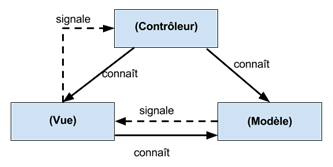
\includegraphics{./img/mvc.png}
    \caption{Patron de conception MVC}
    \label{mvc}
\end{figure}

Le modèle (M) représente les données traitées, dans le cas de l’application ce sont principalement les utilisateurs et leur position GPS. Les deux autres composants n’interagissent pas directement avec les données brutes mais on accès à l’API du modèle symbolisée par le gestionnaire d’utilisateur (UserManager). Le modèle gère donc tous les petits traitements bas niveau sur les données et les sert au reste de l’architecture selon les besoins.

Le contrôleur (C) s’occupe des interactions avec l’utilisateur, il doit pouvoir transmettre les commandes émanant de l’utilisateur aux autres composants.

\subsection{Fonctionnalités introduites}


\subsection{Je ne sais pas}